\chapter {Projekt}
Głównym celem projektu jest stworzenie i weryfikacja modelu rozprzestrzeniania się ognia wykorzystując niehomogeniczne automaty
komórkowe. Nacisk z pracy został położony na opracowanie algorytmu najdokładniej oddającego rzeczywistość.
Aplikacja, nazwa Sparkle została zarojektowana tak, aby zapewnić użytkownikowi wysoką ergonomię pracy i łatwość nauki.
Podczas projektowania i implementacji szczególna uwaga została poświęcona dalszym możliwościom rozbudy programu.
\label{cha:projekt}
\section {Główne zalożenia}
\begin {itemize}
\item Projekt obejmuje zarówno stworzenie modelu rozprzestrzeniania pożaru jak i  uproszczonej wizualizacji oraz graficznego interfejsu użytkownika (GUI).
\item Interfejs aplikacji powinien umożliwiać edycję budynku w którym przeprowadzana jest symulacja: dodawanie elementów konstrukcji, 
określanie materiałów z których zostały stworzone. 
\item Użytkownik powinien mieć możliwość określenia źródła ognia: zarówno jego miejsca jak i temperatury początkowej.
\item Aplikacja powinna umożliwiać także kontrolę nad symulacją: możliwość zatrzymania symulacji, wznowienia, rozpoczęcia od początku,
a także dostosowanie tempa symulacji umożliwiającego obserwację zjawisk fizycznych.
\item Dodatkowym elementem jest zapis wyników w postaci rozkładu temperatu do pliku, umożliwiający dogłębną analizę rezultatów.
\item Wizualizacja powinna obejmować zarówno rozkład temperaturowy jak i rozprzestrzenianie się dymu. 
\end {itemize}
\section {Architektura aplikacji}
% w bibliografi powinno byc coś o tej architekturze i def. aktywnego modelu
Aplikacja została zaprojektowana zgodnie z architekturą Model-View-Controller (w skrócie: MVC).
Rysunek \ref{mvc tradycyjny} przedstawia typowy przykład architektury Model-View-Controller:\\
\begin{figure}
\begin {center}
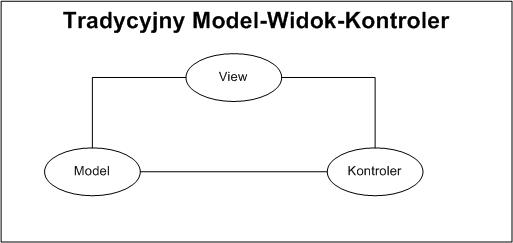
\includegraphics{tradicionalMVC.jpg} \\
\caption { Tradycyjny Model - Widok - Kontroler}
\label {mvc tradycyjny}
%\ref{mvc tradycyjny} %ref do automatycznego odwoływania się
\end {center}
\end{figure}
W omawianej pracy została zaimplementowana pewna odmiana MVC upraszczająca zależności między komponentami.
Najodpowiedniej przedstawia ją schemat: \ref{zmodyfikowany mvc}\\
Uproszczenie zależności między modułami pozwoli niezależnie rozwijać kolejne części aplikacji, w łatwy
sposób podmieniać i modyfikować ich zachowanie.
\begin{figure}
\begin {center}
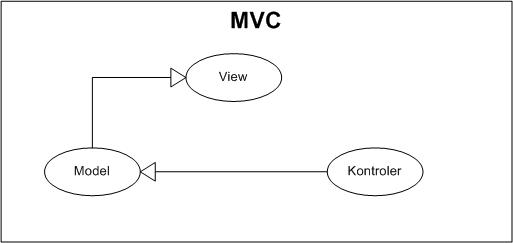
\includegraphics{ourMVC.jpg} \\
\caption { Zmodyfikowany model MVC}
\label {zmodyfikowany mvc}
%\ref{zmodyfikowany mvc} %ref do automatycznego odwoływania się
\end {center}
\end{figure}
Kontroler odpowiada za pobranie danych od użytkownika, ich przetworzenie oraz dostarczenie do modelu.
Został zastosowany przypadek aktywnego modelu, który zgodnie z definicją potrafi zmieniać swój stan 
bez względu na akcje wykonywane przez użytkownika. W projekcie symulacji pożaru aktywność modelu polega na 
wykonywaniu pętli symulacji, związanych z nią obliczeń, powiadamianiu widoku o zachodzących zmianach oraz
końcu symulacji. Widok odpowiada jedynie za prezentację wyników symulacji.
Wybrana architektura umożliwia elastyczny rozwój aplikacji. Wprowadzony podział na trzy odrębne moduły pozwala
na nieograniczone zmiany w każdym z nich, nie powodując konieczności zmian innych części aplikacji.
Inną zaletą separacji jest łatwość testowania poszcególnych modułów osobno. 
\section {Moduły}
\section {Obiekty}
